\documentclass[12pt]{article}
\usepackage[margin=1.5cm]{geometry}
\usepackage{newverbs,listings}
\usepackage[dvipsnames]{xcolor}
\usepackage{tikz}

\usetikzlibrary{arrows,chains,calc,shapes,shapes.multipart,shapes.callouts}

\tikzset{node distance=0,pin distance=9pt}
\tikzstyle{c}=[draw,on chain, minimum height=13pt,minimum width=13pt]
\tikzstyle{a}=[c,fill=yellow]
\tikzstyle{h}=[inner sep=1pt,ellipse,fill=blue!20]
\tikzstyle{p}=[c,fill=SpringGreen,minimum width=40pt]
\tikzstyle{m}=[<->,draw,shorten >=3pt,shorten <=3pt,thin,olive!50!black,fill=white,text=black]
\tikzstyle{u}=[draw,very thick,red,]
\tikzstyle{f}=[draw,blue!50!black,->,shorten <=2pt,shorten >=2pt]
\newenvironment{layout}{\quote\tikzpicture[start chain=going right,x=13pt,y=13pt]\scriptsize}
                       {\endtikzpicture\endquote}
    

\newcounter{segment}
\setcounter{segment}{0}
\newread  \tempFile     % A temporary reading stream
\newwrite \codeFile     % A stream to save the code fragment 

\immediate \openout \codeFile=\jobname.cc

\lstnewenvironment{code}[1][\relax]{\lstset{#1}}{}

    
    
\definecolor{eclipse-purple}{rgb}{0.50,0.00,0.33} % Keyowrds
\definecolor{eclipse-blue}{rgb}{0.16,0.00,1.00} % Doc 
\definecolor{eclipse-green}{rgb}{0.25,0.50,0.37} % Comments
\definecolor{eclipse-red}{rgb}{0.6,0,0} % for strings

\definecolor{clr-background}{RGB}{255,255,255}
\definecolor{clr-text}{RGB}{0,0,0}
\definecolor{clr-string}{RGB}{163,21,21}
\definecolor{clr-namespace}{RGB}{0,0,0}
\definecolor{clr-preprocessor}{RGB}{128,128,128}
\definecolor{clr-keyword}{RGB}{0,0,255}
\definecolor{clr-type}{RGB}{43,145,175}
\definecolor{clr-variable}{RGB}{0,0,0}
\definecolor{clr-constant}{RGB}{111,0,138} % macro color
\definecolor{clr-comment}{RGB}{0,128,0}

 

\lstset{%
    language=C++,
    morekeywords={Constants, Types},
	basicstyle=\color{black}, % any text
	commentstyle=\color{eclipse-green},
	stringstyle=\color{eclipse-red},
	identifierstyle=\color{clr-variable}, % just about anything that isn't a directive, comment, string or known type
	directivestyle=\color{blue}\itshape, % preprocessor commands
	% listings doesn't differentiate between types and keywords (e.g. int vs return)
	% use the user types color
	keywordstyle=\color{clr-type},
	keywordstyle={[2]\color{clr-constant}}, % you'll need to define these or use a custom language
    commentstyle=\itshape,
    keywordstyle=\bfseries\color{eclipse-purple},
    stringstyle=\ttfamily,
    breaklines=true,
    columns={fullflexible},
    texcl=true,
    fontadjust,
    escapechar=`,
    mathescape,
    extendedchars=false,
    showstringspaces=true,
    escapeinside={/*}{*/},
    escapebegin={\works},
}

\begin{document}

\begingroup
\catcode`@=\active
\gdef\works{%    note the global \gdef
  \catcode`@=\active
  \def@##1@{%
        \noindent\textbf{\refstepcounter{segment}\arabic{segment}.~##1.}%
  }%
}%
\endgroup
\begin{code}/* @Primitive types characterizing the machine@ We begin with a %
definition  of the basic types that characterize our presumed JVM like machine 
i.e., byte addressable, two-complement and where words (W) are 32 bits wide, 
half words (H) are 16 bits, and bytes (B) are 8 bits. */
#include <cstdint> // Standard header providing width integer types 

typedef int8_t  B; // A byte, 8 bits 
typedef int16_t H; // Half a word, 16 bits; two bytes
typedef int32_t W; // A full word of 32 bits; four bytes, two half words
\end{code}

\begin{code}
/* @S-Expressions and  handles@ An S-expression is either a  dotted pair 
(consistuted by two, smaller, S-expressions) or an atom (which is a string of 
characters.  An S-expression is represented by a 16 bits handle (the 
type H) encoding an integer $h$,
\[2^{15} \le h \le 2^{15}-1\] 

The handle of a dotted pair is always positive. The handle of the 
special atom  NIL is zero; handles of all other atoms are negative. The sign bit 
of a handle is therefore 
a boolean: if it set, then the handle is an atom.
*/
struct S { // handle of S expression
  H h; // the handle
};
/*
A handle makes it possible access the representation of the actual data: in the case
of an  expression.
*/
\end{code}

\begin{code}
/* @Represenation of atoms@ Also, for the purpose of our implementation we
represent ``atoms'' (A) as the address of the first byte in sequence of bytes that
end in the null byte, i.e., a byte in which all bits are zero, denoted in C by \verb/'\0'/ and mathematically by~$\natural$. 
\[
\verb/'\0'/ = \natural= 
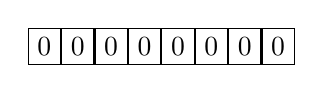
\begin{tikzpicture}[start chain=going right]
\foreach \i in {1,...,8} \node [draw,on chain] {0};
\end{tikzpicture}
\]
*/

typedef const B *const A; // Underlining representation of strings as pointers to bytes  
\end{code}

\begin{code}/* @Representation of a dotted pair@ A dotted pair (for short, ``pair'') is 
an unlabeled internal node in the binary tree representation of an S-expression. 
A pair is stored in a word containing two half words. The car and the cdr parts 
of the node. We also pairs to make linked lists, where one half word is the
contents of a list item, and the other is a pointer to the subsequent item.
*/
union Pair { // The perspectives of a pair.
  W cons: 32;                   // I. A single word that can 
  struct { H car, cdr:16 };    // II. A pair of car and cdr, each in a word.
  struct { H data, next:16};   // III. An item in a linked list
};
\end{code}

\begin{code}
/* @Handles as indices@ An S-expresion is either a %
dotted pair (consistuted by two, smaller, S-expressions) or an atom. %
Such an expression is represented by a half-word that represents an integer $h$, %
\[2^{15} \le h \le 2^{15}-1\] 
\begin{description}
    \item[Dotted Pairs] If $h>0$, then the S-experssion that $h$ represents is a %
    dotted-pair. The value of $h$ is interpeted as an index in the pairs' pool: %
    an array $P$ of pairs whose indices are in the range $1,2,\ldots p$, and %
    where $p>0$ is the number of pairs in the the statically allocated %
    memory block used for storing pairs. %
\begin{layout}
\foreach \i in {1,...,3} \node[p] (p\i) [pin=above:{\i}] {};
\node[p] (p4) [minimum width=120pt] {$\cdots$};
\node[p] (p5) [p,pin=above:{$n_p-1$}] {};
\node[p] (p6) [p,pin=above:{$n_p$}] {};
\node (label) [above=2 of p4]{\bf Pairs' Pool ($1\le h\le p$)};
\foreach \n/\l/\p in { P0/$P_0=P$/p1.north west,P1/$P_1=P+4p$/p6.north east} 
%    \node(\n) [below=3 of \p] {\l} edge[u] (\p |+ label); 
    \node(\n) [below=3 of \p] {\l} edge[u] ($(\p)+(0,3)$); 
    \path [u] (P0) -- +(0,1) coordinate (B0);
    \path [u] (P1) -- +(0,1) coordinate (B1);
    \draw[m] ($(P0)+(0,1)$)-- node (B) [fill=white,text=black] {$p$ pairs ($4p$ bytes)} ($(P1)+(0,1)$) ;
\end{layout}
    \item[Atoms] If $h\le0$, then this S-expression is an atom. 
     The value of case $h$ is interpeted as a, typically negative, index into 
     the atoms' pool, an array $A$ of $a$ bytes, whose indices are in the 
     range \[
            -a+4,-a+3,\ldots,0,\ldots,3
    \]  where $a$ is some fixed contant. In other words, $A$ is some fixed 
    memory address, used to acces a memory block of $a$ bytes that ranges 
    from address $A_0=A-a+1$ to address $A_1=A+3$
\begin{layout}
\node[a] (a0) [pin=above:{$-a+4$}] {};
\node[a] (a1) [minimum width=56ex] {$\cdots$};
\foreach \i/\l[count=\j from -8] in {ndefun/\tt N,defun/\tt D,/\tt E,/\tt F,/\tt U,/\tt N,/$\natural$,t/\tt T,12/$\natural$,nil/\tt N,10/\tt I,11/\tt L,a$/$\natural$} \node (\i) [a,pin=above:{\tiny \j}] {\l};
\path ($(a1)!0.5!(a$)$) ++(0,3)  node {\bf Atoms' Pool ($-a+4 \le h\le 0$)};

    \node(A0)  [below=4 of a0.south west] {$A_0=A-a+4$}; 
    \node(A)   [below=2 of nil.south west] {$A$}; 
    \node(A1)  [below=4 of a$.south east] {$A_1=a+3$};
    \draw[u] (A0) -- +(0,9);
    \draw[u] (A) -- +(0,4);
    \draw[u] (A1) -- +(0,9);
    \draw[m] ($(A0)+(0,1)$)--node(B)[fill=white,text=black]{$a$ bytes}($(A1)+(0,1)$);
    \draw[m] ($(A0)+(0,3)$)--node(B)[fill=white,text=black]{$a$ bytes}($(A)+(0,1)$);
    \draw[m] ($(A)+(0,1)$)--node(B)[fill=white,text=black]{$4$ bytes}($(A1)+(0,3)$);
    
    \node[below=8 of nil,h]{\tt nil} edge [f] node[above,rotate=90,very near start] {\tiny $h=0$} (nil);
    \node[below=7 of t,h] {\tt t} edge[f] node[above,rotate=90,very near start] {\tiny $h=-1$} (t);
    \node[below=10 of defun,h] {\tt defun} edge [f] node[above,rotate=90,very near start] {\tiny $h=-7$} (defun);
    \node[below=7 of ndefun,h] {\tt ndefun} edge[f] node[above,rotate=90,near start] {\tiny $h=-8$} (ndefun);


%\foreach \n/\l/\p in { A0//a1.north west,A0/$A_0=A-a+4$/a1.south west,A/$A$/nil.north west,//a$.north east,A1/$A_1=A+3$/a$.south east} 
   %\node(\n) [below=3 of \p] {\l} edge[u] ($(\p)+(0,1)$); 
    %\path [u] (P0) -- +(0,1) coordinate (B0);
    %\path [u] (P1) -- +(0,1) coordinate (B1);
\end{layout}
\end{description}
\end{code}

\begin{itemize}
    \item  integers 
    \emph{Positive integers}
Positive integer designates a * 
pair, i.e., an internal node; a negative pair represents a string. A zero
 * integer designates the NIL atom.  There is a bit of trickery to make sure
 * that if the index zero, the string behind it happens to be NIL. In a sense
 * the zero is also an index into the strings array.
 *
 * Both pools are consecutive in memory: There is a large static buffer in which 
 * both pools reside.
 */
\end{itemize}



\begin{code}[literate=
    {=}{$\equiv$ }{1}
    {*}{$\times$}{1}
    {1<<$H_c$}{$2^{H_c}$}{3}
]
/* @Sizes of related to primitive types@*/
Constants {
    $B_n$ = 8*sizeof B,    // Eight bits in byte
    $H_n$ = 8*sizeof H,    // Sixteen bits in a half word
    $W_n$ = 8*sizeof W,    // Thity-two bits in a full word
    
    $H_c$ = $H_n$ - 1,     // Number of bits in the characteristic of type H
    $H_x$ = 1<<$H_c$       // Maximal positive value representable in type H
}
\end{code}

\begin{code}[literate=
    {*}{$\times$}{1}
    {=}{$\equiv$ }{1}{*}{$\times$}{1}
    {1<<13}{$2^{13}$}{3}
    {1<<15}{$2^{15}$}{3}
    {1a<<$H_x$}{$2^{H_x}$}{3}
]
/* @Static memory@ 
All memory allocations are from a pre-allocated fixed 
contigious memory block, the \emph{pool} of $n$ bytes comprising:
\begin{enumerate} 
\item \emph{Pool of atoms}. A sub-block $N_1$ \emph{bytes}, from which 
internal representations of atoms are allocated. 
\item \emph{Pool of pairs}. A sub-block $n_2$ \emph{words},
from which internal representations of pairs are allocated. 
\end{enumerate}

\begin{layout}
\node[a] (a1) [pin=below:$-n_1+4$]{};
\node[a] (a2) {};
%\node[a] (a3) {};
\node[a] (a4) [minimum width=45pt] {$\cdots$};
\foreach \i/\l[count=\j from -4] in {5/,6/,7/T,8/$\natural$,9/N,10/I,11/L,12/$\natural$} \node (a\i) [a,pin=below:{\j}] {\tt\l};

\foreach \i in {1,...,3} \node[p] (p\i) [pin=below:{\i}] {};
\node[p] (p4) [minimum width=160pt] {$\cdots$};
\node[p] (p5) [p,pin=below:{$n_2-1$}] {};
\node[p] (p6) [p,pin=below:{$n_2$}] {};

\node[above=of a4] { \bf other atoms };
\node[p,draw,fill=olive!30,above=of nil.north west,anchor=south west,pin=above:0] { \bf nil };
\node[p,draw,fill=olive!30,above=of p1,pin=above:1] {};
\node[p,draw,fill=olive!30,above=of p2,pin=above:2] {};
\node[p,draw,fill=olive!30,above=of p3,pin=above:2] {};
\node[p,draw,fill=olive!30,above=of p4,minimum width=160pt] {};
\node[p,draw,fill=olive!30,above=of p5,pin=above:$n_2-1$] {};
\node[p,draw,fill=olive!30,above=of p6,pin=above:$n_2$] {};

\draw[ultra thick,blue] (a1.south west)-- (a1.north west)--++(0,30pt) ++(0,-5pt) coordinate (T1);
\draw[ultra thick,blue] (nil.south west)--(nil.north west)-- ++(0,30pt) ++(0,-5pt) coordinate (T2);
\draw[ultra thick,blue] (p1.south west)--(p1.north west)-- ++(0,30pt) ++(0,-5pt) coordinate (T3);
\node (N4) at ($(T1)!0.5!(T2)$) {\it$n_1-4$ bytes};

\draw[m] (N4) -> (T1);
\draw[m] (N4) ->(T2);
\draw[ultra thick,blue] (a1.south west) -- ++(0,80pt) ++(0,-20pt) coordinate (P1);
\draw[ultra thick,blue] (p1.south west) -- ++(0,80pt) ++(0,-20pt) coordinate (P2);
\draw[ultra thick,blue] (p6.south east) -- ++(0,80pt) ++(0,-20pt) coordinate (P3);
\node (N1) at ($(P1)!0.5!(P2)$) {\it$n_1$ bytes};
\node (N2) at ($(P2)!0.5!(P3)$) {\it$n_2$ words};
\draw[m] (N1) -> (P1);
\draw[m] (N1) ->(P2);
\draw[m] (N2)->(P2);
\draw[m] (N2)->(P3); 
\node(L2) [above=of N2]  {\bf Pool of pairs}; 
\node(L1) [above=of N1]  {\bf Pool of atoms}; 

\draw[ultra thick,blue] (P1) --++(0,-110pt)++(0,5pt) coordinate (Q1) (P3) --++(0,-110pt)++(0,5pt) coordinate(Q2);
\node (N) at ($(Q1)!0.5!(Q2)$) {\tiny\bf $N$ bytes };
\node (P) [above=of N] {\bf\scriptsize Static Memory} ;
\draw[m]  (N) ->(Q1);
\draw[m] (N) ->(Q2);
\end{layout}
*/ 
Constants {
    $N_1$ = 1<<13,
    $N_2$ = 1<<15 -1,    
    $N$ = $N_1$*sizeof B + $N_2$*sizeof W,    
}

static B M[N]; 
\end{code}


\end{document}
